\documentclass{article}

% if you need to pass options to natbib, use, e.g.:
% \PassOptionsToPackage{numbers, compress}{natbib}
% before loading nips_2018

% ready for submission
%\usepackage{nips_2018}

% to compile a preprint version, e.g., for submission to arXiv, add
% add the [preprint] option:
\usepackage[preprint]{nips_2018}

% to compile a camera-ready version, add the [final] option, e.g.:
% \usepackage[final]{nips_2018}

% to avoid loading the natbib package, add option nonatbib:
% \usepackage[nonatbib]{nips_2018}
% For citations

\usepackage[utf8]{inputenc} % allow utf-8 input
\usepackage[T1]{fontenc}    % use 8-bit T1 fonts
\usepackage{hyperref}       % hyperlinks
\usepackage{url}            % simple URL typesetting
\usepackage{booktabs}       % professional-quality tables
\usepackage{amsfonts}       % blackboard math symbols
\usepackage{nicefrac}       % compact symbols for 1/2, etc.
\usepackage{microtype}      % microtypography
\usepackage{graphicx}
\usepackage{placeins}
\usepackage{subcaption}
\usepackage{float}

% For algorithms
\usepackage{algorithm}
\usepackage{algorithmic}
\usepackage{amsfonts}
\usepackage{amstext}
\usepackage{amssymb}
\usepackage{amsmath}

\title{Explanations for Multinomial Classifiers\\\vspace{10pt}\small{Tips and Tricks for Practitioners}}

% The \author macro works with any number of authors. There are two
% commands used to separate the names and addresses of multiple
% authors: \And and \AND.
%
% Using \And between authors leaves it to LaTeX to determine where to
% break the lines. Using \AND forces a line break at that point. So,
% if LaTeX puts 3 of 4 authors names on the first line, and the last
% on the second line, try using \AND instead of \And before the third
% author name.

% Authors in alphabetical order
\newcommand*\samethanks[1][\value{footnote}]{\footnotemark[#1]}
\author{
  Pramit Choudhary\thanks{H2O.ai}\\
  Mountain View, CA\\
  \texttt{pramit.choudhary@h2o.ai}\\
  \And
  Navdeep Gill\samethanks\\
  Mountain View, CA\\
  \texttt{navdeep.gill@h2o.ai}\\ 
  \And
  Patrick Hall\thanks{H2O.ai and George Washington University}\\
  Washington, DC\\
  \texttt{patrick.hall@h2o.ai}}

\begin{document}

\maketitle

\begin{abstract}


\end{abstract}

\section{Introduction}

This short discussion bookends popular and practical texts on machine learning explanations by Choudhary, Gill, Hall et al. by specifically addressing the common and somewhat vexing problem of explaining the behavior and predictions of supervised multinomial classifiers \cite{oreillymli}, \cite{art_and_sci}, \cite{oreillyskater} \cite{sarkar2018practical}. This paper is a continuation of ongoing research and our understanding of various techniques that are useful to understand a complex "black box" model's decision policies.

%Difficulty of knowing if explanations are "right" -- this is why we chose simulated data.

%-------------------------------------------------------------------------------
\section{Notation} \label{sec:notation}
%-------------------------------------------------------------------------------

To facilitate technical descriptions of explanatory techniques, notation for input and output spaces, datasets, and models is defined.

\subsection{Spaces} 
 
	\begin{itemize}
		\item Input features come from the set $\mathcal{X}$ contained in a \textit{P}-dimensional input space,\\ $\mathcal{X} \subset \mathbb{R}^P$.  
		\item Known labels corresponding to instances of $\mathcal{X}$ come from the set $\mathcal{Y}$ contained in a \textit{C}-dimensional input space, $\mathcal{Y} \subset \mathbb{R}^C$.
		\item Learned output responses come from the set $\hat{\mathcal{Y}}$. For classification models the set $\hat{\mathcal{Y}}$ typically contains a column vector for each unique class in $\mathcal{Y}$. In this text, the space $\hat{\mathcal{Y}}$ is said to be contained in a $C'$-dimensional output space,  $\hat{\mathcal{Y}} \subset \mathbb{R}^{C'}$. 
%		\item The output responses come from a set $\mathcal{Y}$ contained in a $C$-dimensional output space (i.e. $\mathcal{Y} \subset \mathbb{R}^C$).
	\end{itemize}	
	
	\subsection{Datasets} 

	\begin{itemize}
		\item The input dataset $\mathbf{X}$ is composed of observed instances of the set $\mathcal{X}$ with a corresponding dataset of labels $\mathbf{Y}$, observed instances of the set $\mathcal{Y}$.
		\item Each $i$-th observation of $\mathbf{X}$ is denoted as $\mathbf{x}^{(i)} = $  
		$[x_0^{(i)}, x_1^{(i)}, \dots, x_{\textit{P}-1}^{(i)}]$, with corresponding $i$-th labels in $\mathbf{Y}, \mathbf{y}^{(i)} = [y_0^{(i)}, y_1^{(i)}, \dots, y_{\textit{C}-1}^{(i)}]$, and corresponding predictions in $\mathbf{\hat{Y}}, \mathbf{\hat{y}}^{(i)} =  [\hat{y}_0^{(i)}, \hat{y}_1^{(i)}, \dots, \hat{y}_{\textit{C'}-1}^{(i)}]$. % = [y_0^{(i)}, y_1^{(i)}, \dots, y_{\textit{C}-1}^{(i)}]$.
		\item $\mathbf{X}$ and $\mathbf{Y}$ consist of $N$ tuples of observations: $[(\mathbf{x}^{(0)},\mathbf{y}^{(0)}), (\mathbf{x}^{(1)},\mathbf{y}^{(1)}), \dots,$\\$(\mathbf{x}^{(N-1)},\mathbf{y}^{(N-1)})]$. %\\ $\mathbf{x}^{(i)} \in \mathcal{X}$, $\mathbf{y}^{(i)} \in \mathcal{Y}$.
		\item Each $j$-th input column vector of $\mathbf{X}$ is denoted as $X_j = [x_{j}^{(0)}, x_{j}^{(1)}, \dots, x_{j}^{(N-1)}]^T$.
	\end{itemize}	
	
	\subsection{Models}

	\begin{itemize}
		\item A type of machine learning model $g$, selected from a hypothesis set $\mathcal{H}$, is trained to represent an unknown signal-generating function $f$ observed as  $\mathbf{X}$ with labels $\mathbf{Y}$ using a training algorithm $\mathcal{A}$: 
		%\\ $\mathbf{X}, \mathbf{Y} \xrightarrow{\mathcal{A}} g$.
		\item $g$ generates learned output responses on the input dataset $g(\mathbf{X}) = \mathbf{\hat{Y}}$, and on the general input space $g(\mathcal{X}) = \hat{\mathcal{Y}}$.
		\item The model to be explained is denoted as $g$.
	\end{itemize}

%\section{Simulated Data Experiments}

\section{Global Analysis}

\subsection{Data}
Subsequent sections will use simulated data to empirically demonstrates the desired relationships and interaction between input feature space $\mathbf{X}$, the output space $f(\mathbf{X}) = \mathbf{Y}$. Simulated data is generated using a pre-defined signal-generating function using four input features with interactions and with eight noisy features with ground truth containing three unique categories(class 1, class 2, class 3) as defined below,
\begin{equation}
\label{eq:f}
f = \text{num} _1 * \text{num}_4 + |\text{num}_8| * \text{num}_9^2 + e
\end{equation}

A $g_{\text{GBM}}$ is trained as the base estimator to learn the patterns represented using multinomial logloss as the optimization function and softmax is used to generate the final predictions. 
$ \mathbf{X}, \mathbf{f(X)} \xrightarrow{\mathcal{A}} g_{\text{GBM}}$ such that $g_{\text{GBM}} \approx f$. 

\begin{table}[H]
  \caption{Summarizing evaluation during model training on the simulated dataset}
  \label{eval-table}
  \centering
  \begin{tabular}{lll}
    \toprule
    \cmidrule{1-2}
    Dataset /Number of rows    & F1-score     & log-loss  \\
    \midrule
    Training set(20946) &  0.79 & 0.56     \\
    Test set(9054)     &  0.70 & 0.71      \\
    \bottomrule
  \end{tabular}
\end{table}
** The performance metric reference in the \ref{eval-table} is for completeness. The goal of the paper is not to highlight the building the best possible model.

\subsection{Interpretation via Decision Tree Surrogate} \label{sec:surrogate_dt}
Given a learned function $g$ and a set of learned output responses $g(\mathbf{X}) = \mathbf{\hat{Y}}$, a surrogate decision tree(SDT) $h_{\text{tree}}$ can be constructed to extract comprehensible and faithful concepts such that $h_{\text{tree}}(\mathbf{X}) \approx g_{\text{GBM}}(\mathbf{X}) \approx f(\mathbf{X})$:

\begin{equation}
\mathbf{X}, g(\mathbf{X}) \xrightarrow{\mathcal{A}} h_{\text{tree}}
\end{equation}

\begin{figure}[H]
	\begin{subfigure}[tb]{.5\textwidth}
		\begin{center}
			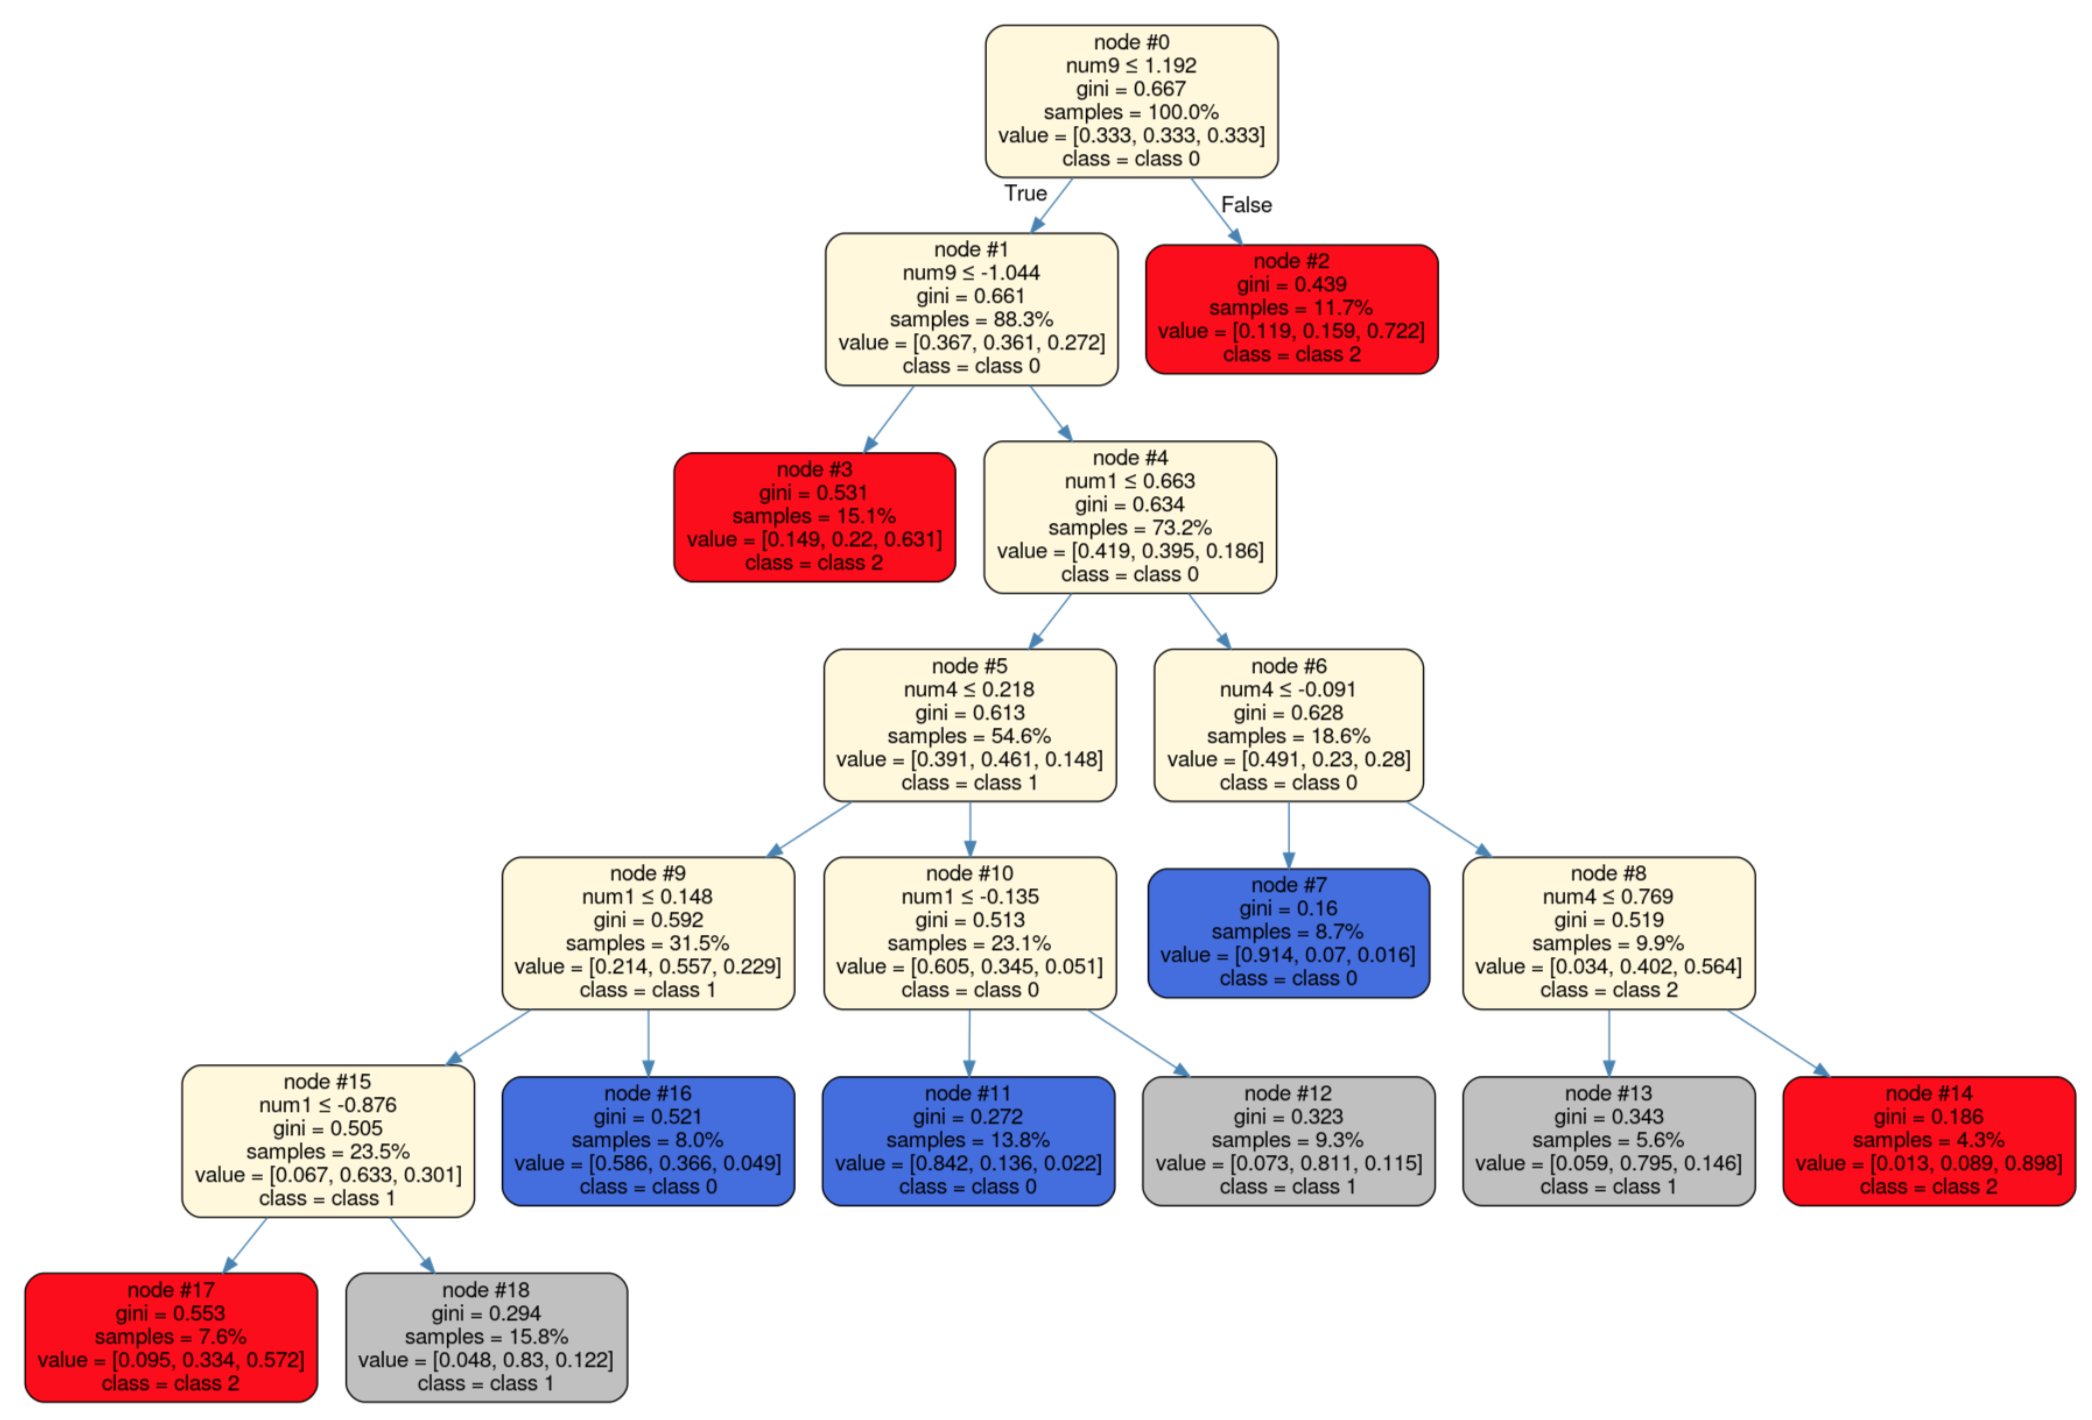
\includegraphics[width=\linewidth]{img/sdt_visualization}
			\caption{}
			\label{fig:surrogate_dt}
		\end{center}
	\end{subfigure}%
	\begin{subfigure}[tb]{.5\textwidth}
		\begin{center}
			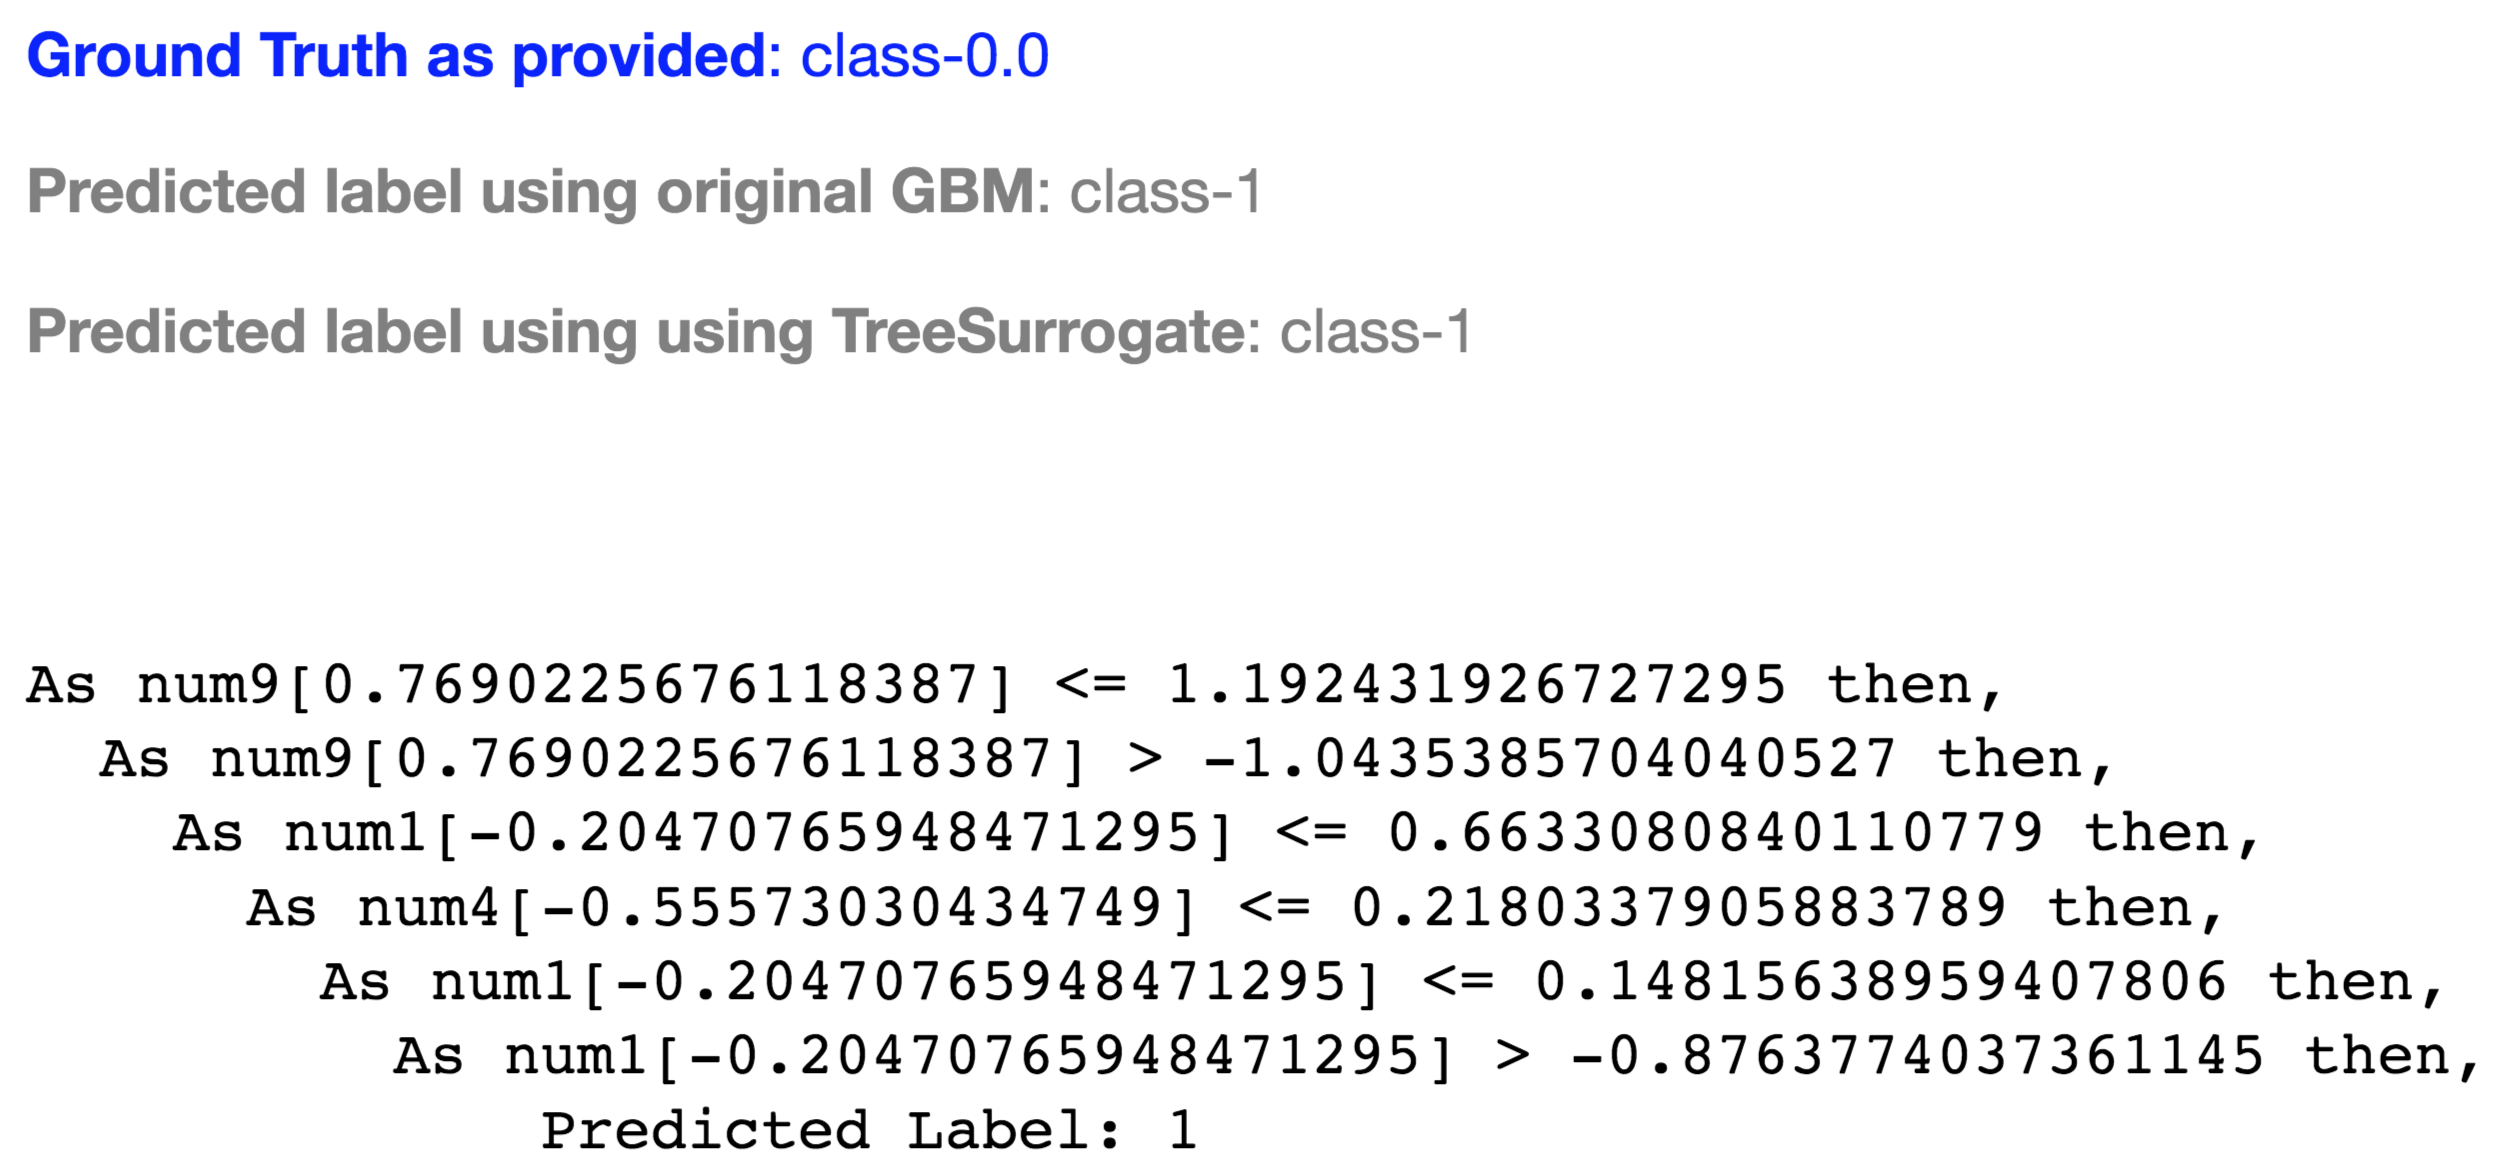
\includegraphics[width=1.3\linewidth]{img/decision_stumps_txt}
			\caption{}
			\label{fig:surrogate_dt}
		\end{center}
	\end{subfigure}%
	\captionsetup{font=footnotesize}
	\caption{\textbf{a:} Illustrates the surrogate decision tree built using the original estimator $g_{\text{GBM}}$. Only the leaf nodes are colored, clearly highlighting class membership. The non-leaf nodes highlights the important features(namely num1, num4, 
	num9) which matches the results computed using the Shapely feature importance. \textbf{b:} Visualizes the decision stumps as a convenient text representation. The decision stumps highlight the rules learned by the SDT for a single input row. The nested 
	"As-then" conditions contain the globally important features(num9, num1, num4). The ground truth for referenced input row is \textit{"class-0"} but both the original model $g_{\text{GBM}}$ and explanation model $h_{\text{tree}}$ predicted \textit{"class-1"}.
	Since, the explanation model has learned the original model's policies concisely, the explanations produced are a faithful approximate representation of the $g_{\text{GBM}}$}
\end{figure}

In the above mentioned learning task, the target labels are derived from the previously learned GBM response function $g_{\text{GBM}}$. \cite{dt_surrogate1} \cite{dt_surrogate2} provide detained information for training a tree surrogate $h_{\text{tree}}$. 
\subsubsection{Recommendations}
\begin{itemize}
\item In order to prevent SDT from creating overly complex un-interpretable "if-then-else" rules that do not generalize well, pruning(pre-pruning with cross validation or post-pruning by optimizing on the multi-class evaluation metic - e.g. f1-score, categorical cross entropy) can be applied to build stable trees.
\item SDT can elegantly handle high cardinality targets maintaining high level of fidelity and faithfulness to the original  estimator function $g$). The faithfulness of the decisions generated by SDT depends on how precisely the tree surrogates captures the decisions learned by the original estimator.
\item Remember to handle class imbalance before fitting a SDT using an oversampling technique - e.g. Synthetic Minority Over-sampling Technique(SMOTE) \cite{chawla2002smote}, Adaptive synthetic sampling approach for imbalanced learning(ADASYN)\cite{he2008adasyn}
\end{itemize}

\subsection{Interpretation via Decision Boundary Plots}
Decision Boundaries is a hypersurface which provides informative interpretation to understand the characteristics of multiclass predictive model by visualizing the distances of the data elements to a model's learned decision plane. The boundary helps in providing a direct reference to the complexity of a classifier and the dataset \cite{rao1997visualizing} \cite{migut2015visualizing}. Figure 2 (a) and (d) illustrates different decision boundaries constructed using a GBM(Gradient Boosted Machine) and a MLP(Mulit-layer Perceptron classifier).
Such representation provides global interpretation using the two or three dimensional feature vector $X$,
\begin{align}
    X &= \begin{bmatrix}
           x_{1} \\
           x_{2} \\
         \end{bmatrix}
\end{align}

\begin{figure}[H]
	\begin{subfigure}[tb]{.5\textwidth}
		\begin{center}
			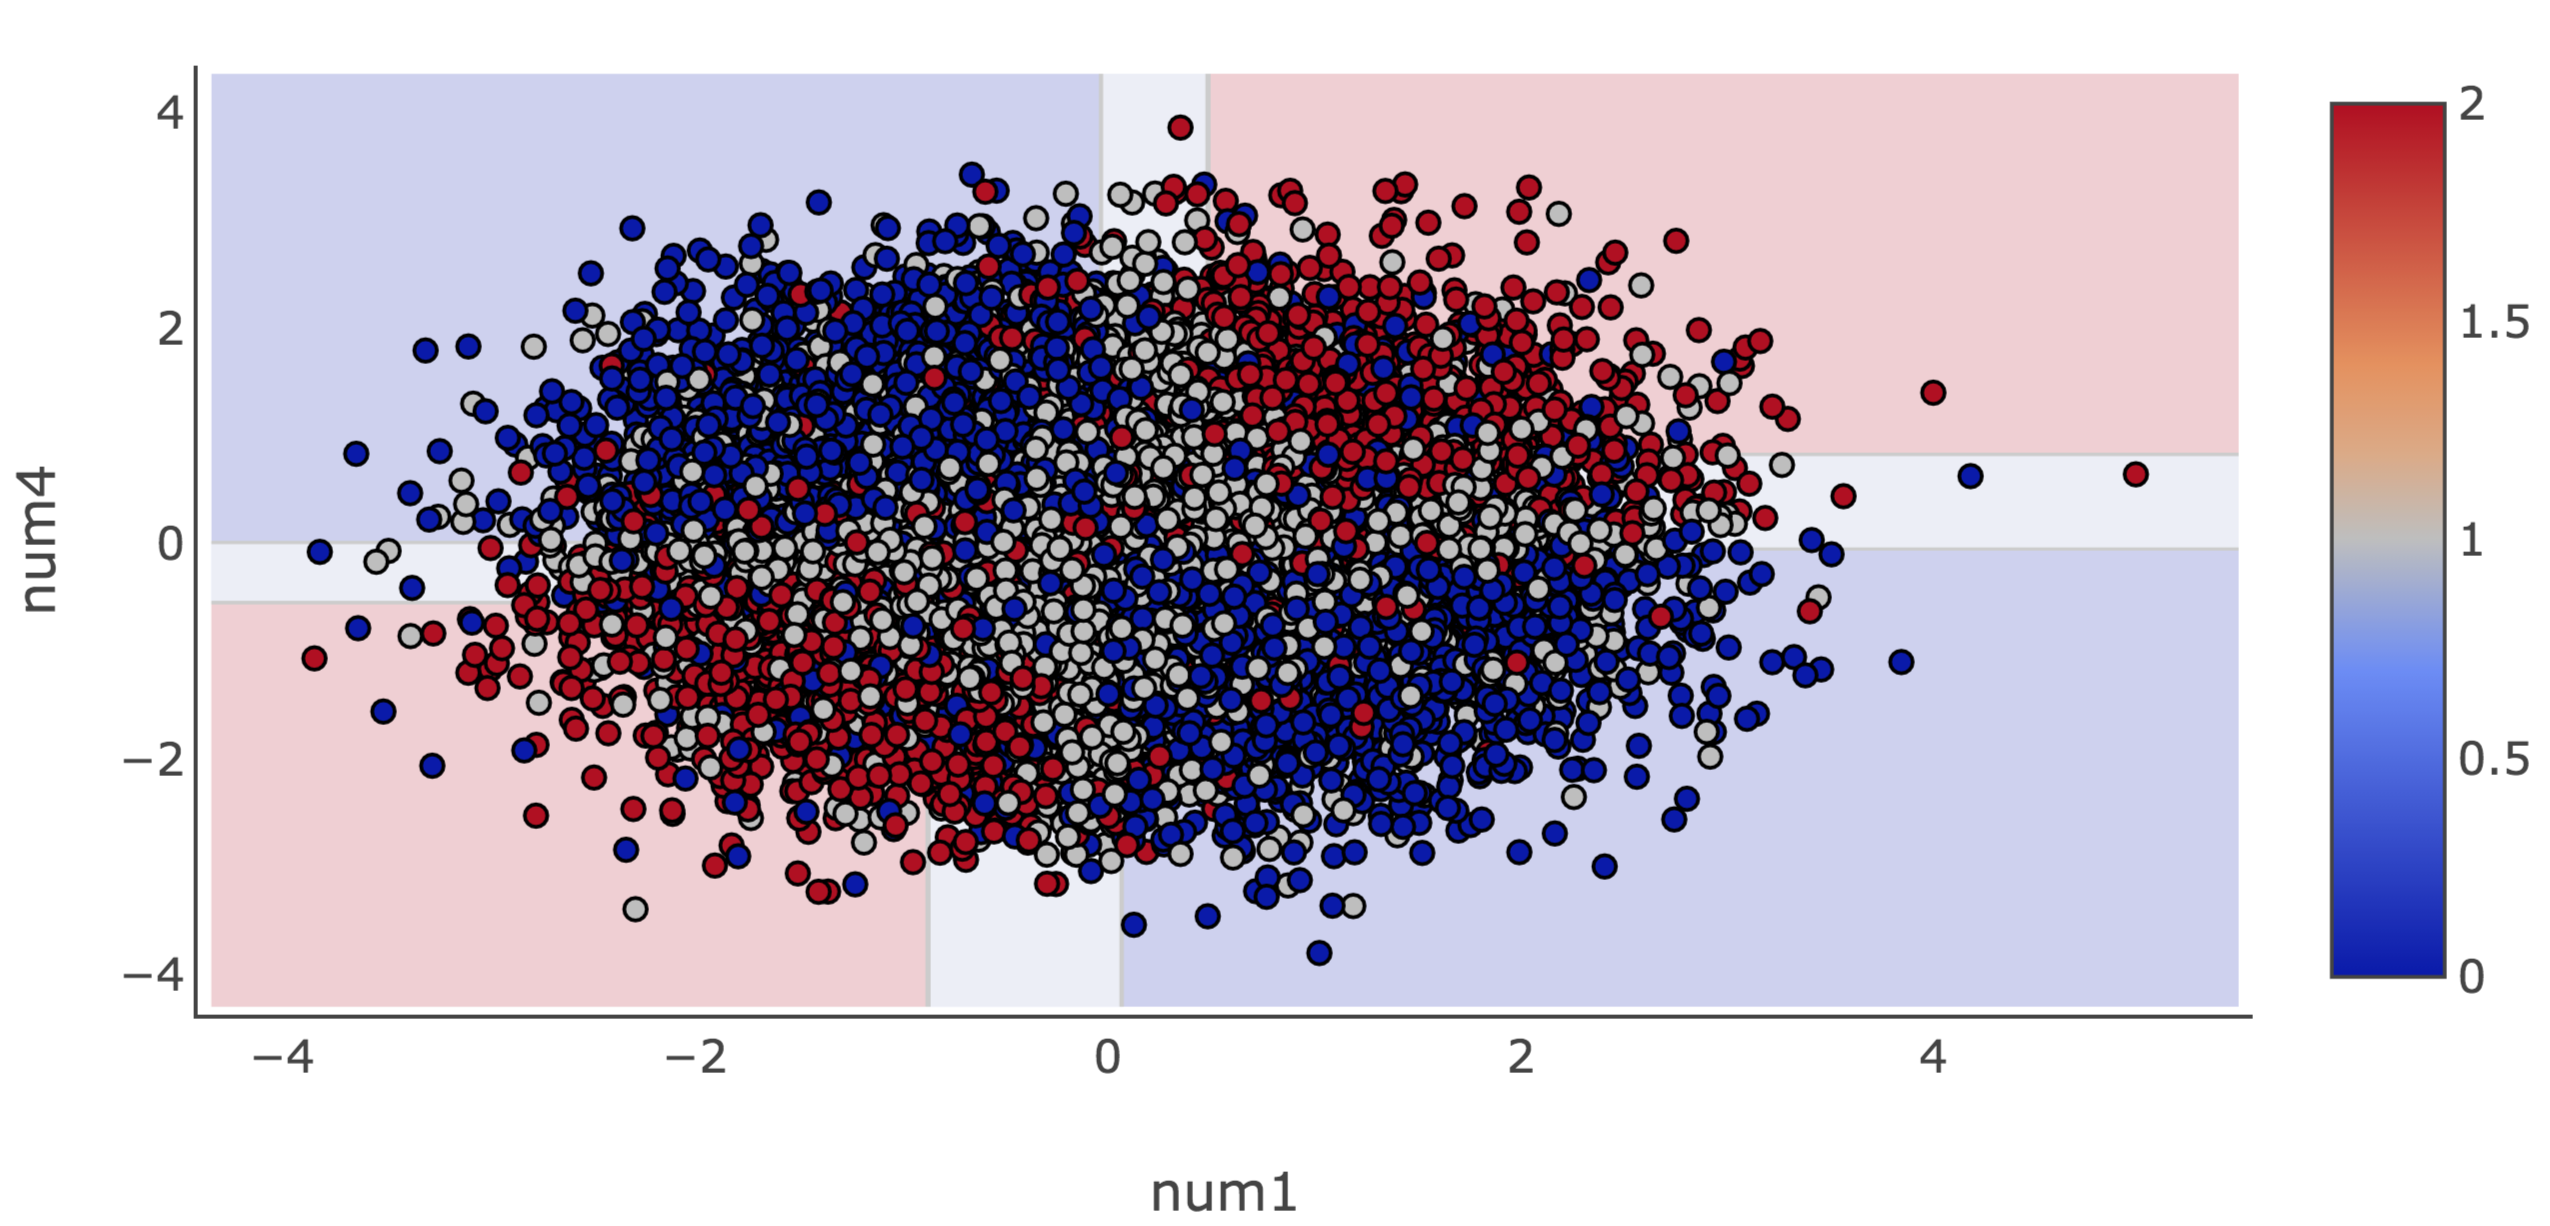
\includegraphics[width=\linewidth]{img/db_num1_num4}
			\caption{}
			\label{fig:global_db}
		\end{center}
	\end{subfigure}%
	\begin{subfigure}[tb]{.5\textwidth}
		\begin{center}
			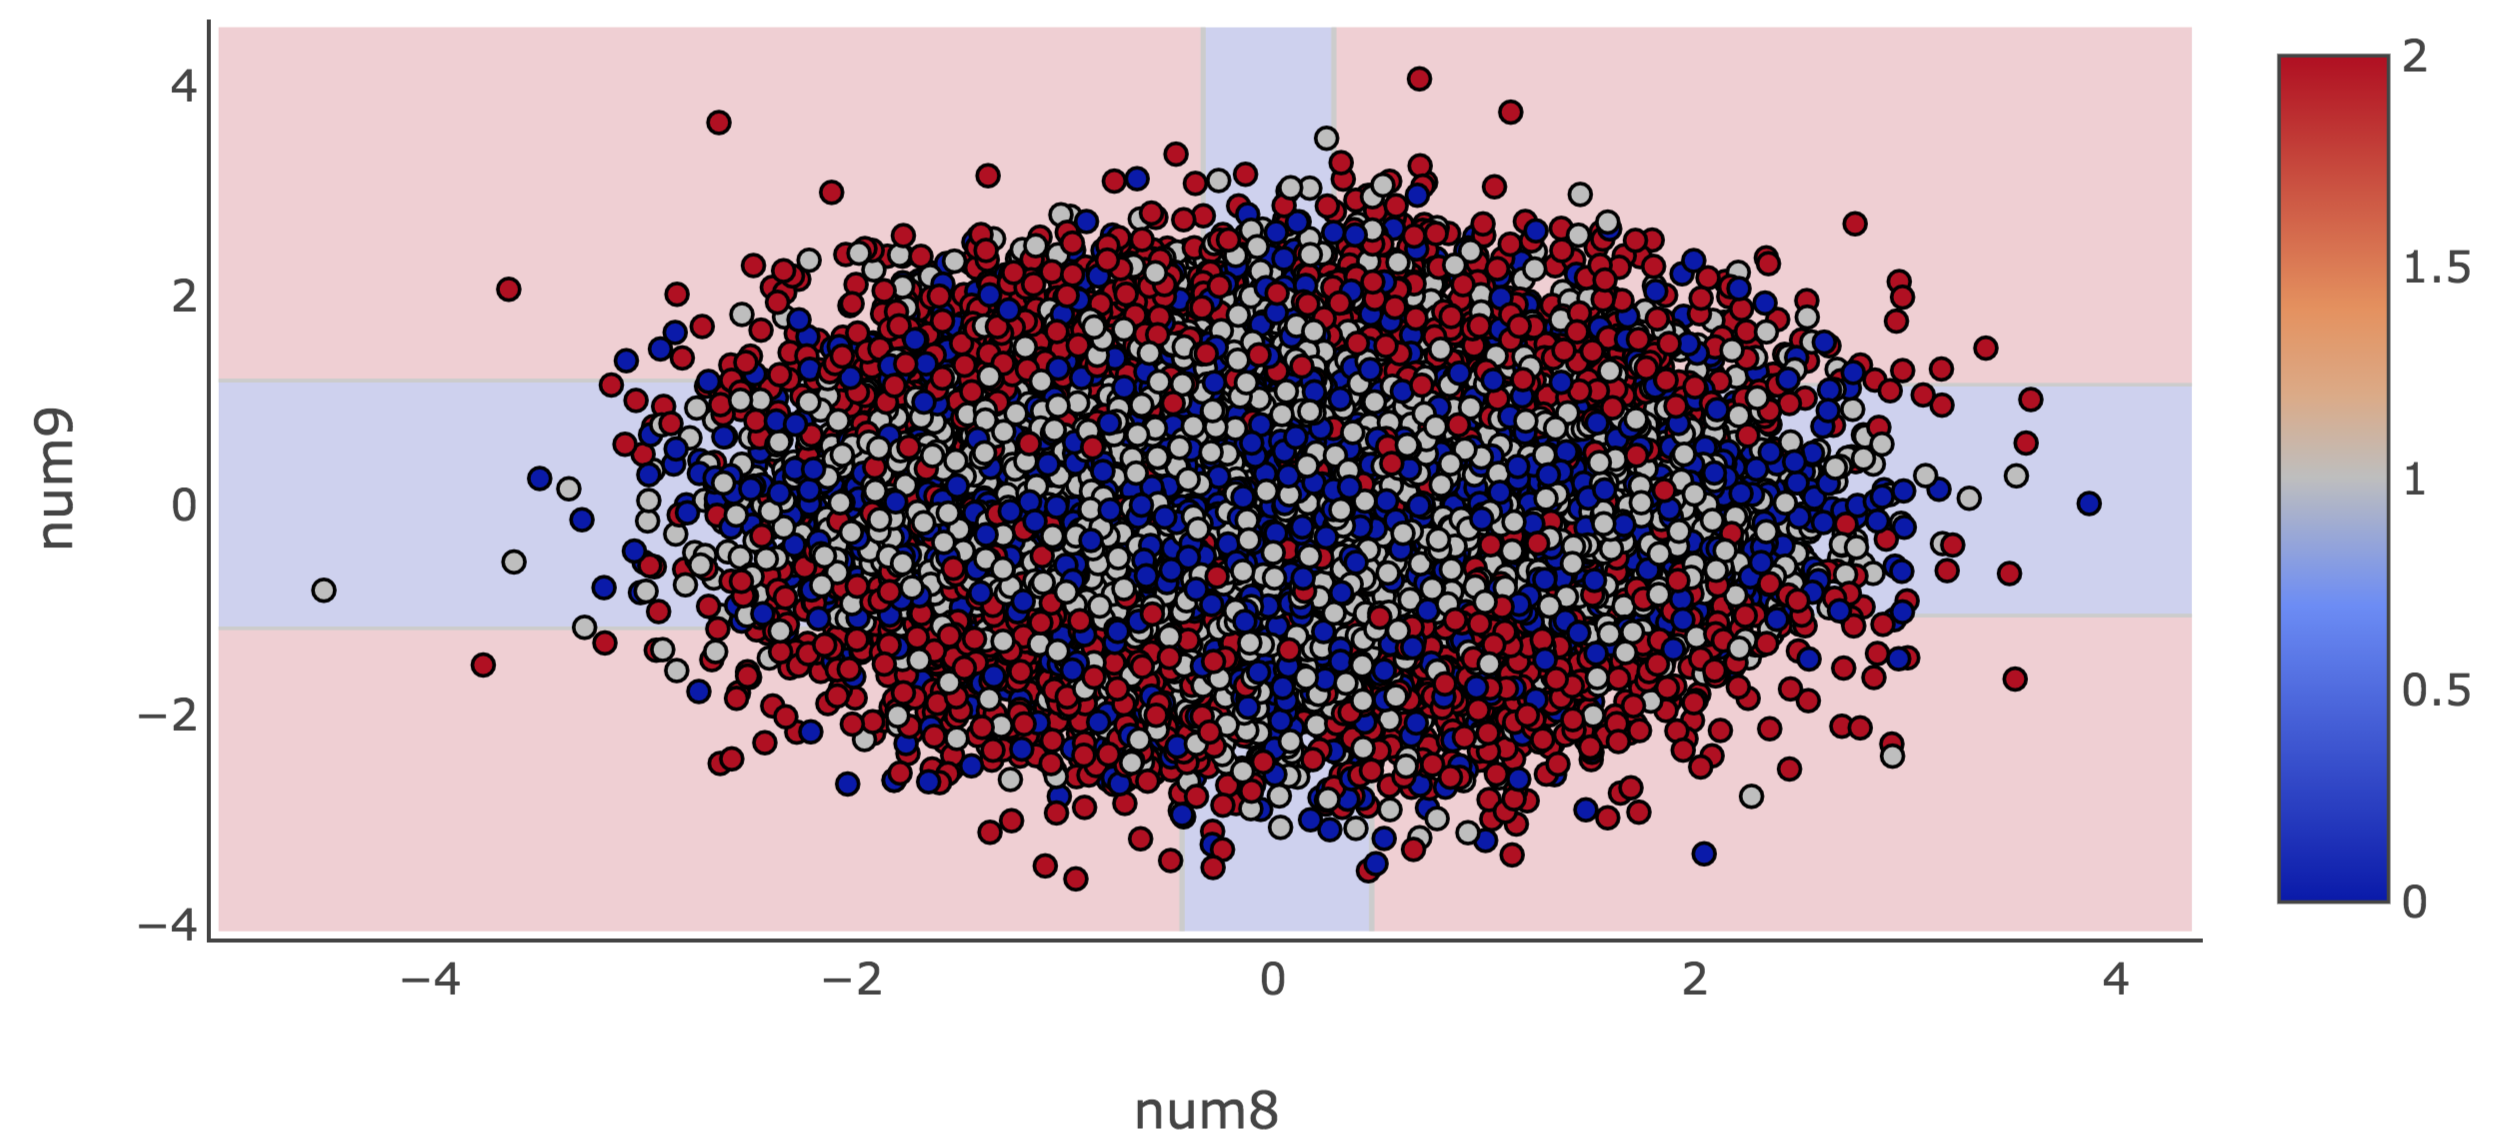
\includegraphics[width=\linewidth]{img/db_num_8_num9}
			\caption{}
			\label{fig:global_db}
		\end{center}
	\end{subfigure}%
	\vskip\baselineskip
	\begin{subfigure}[tb]{.5\textwidth}
		\begin{center}
			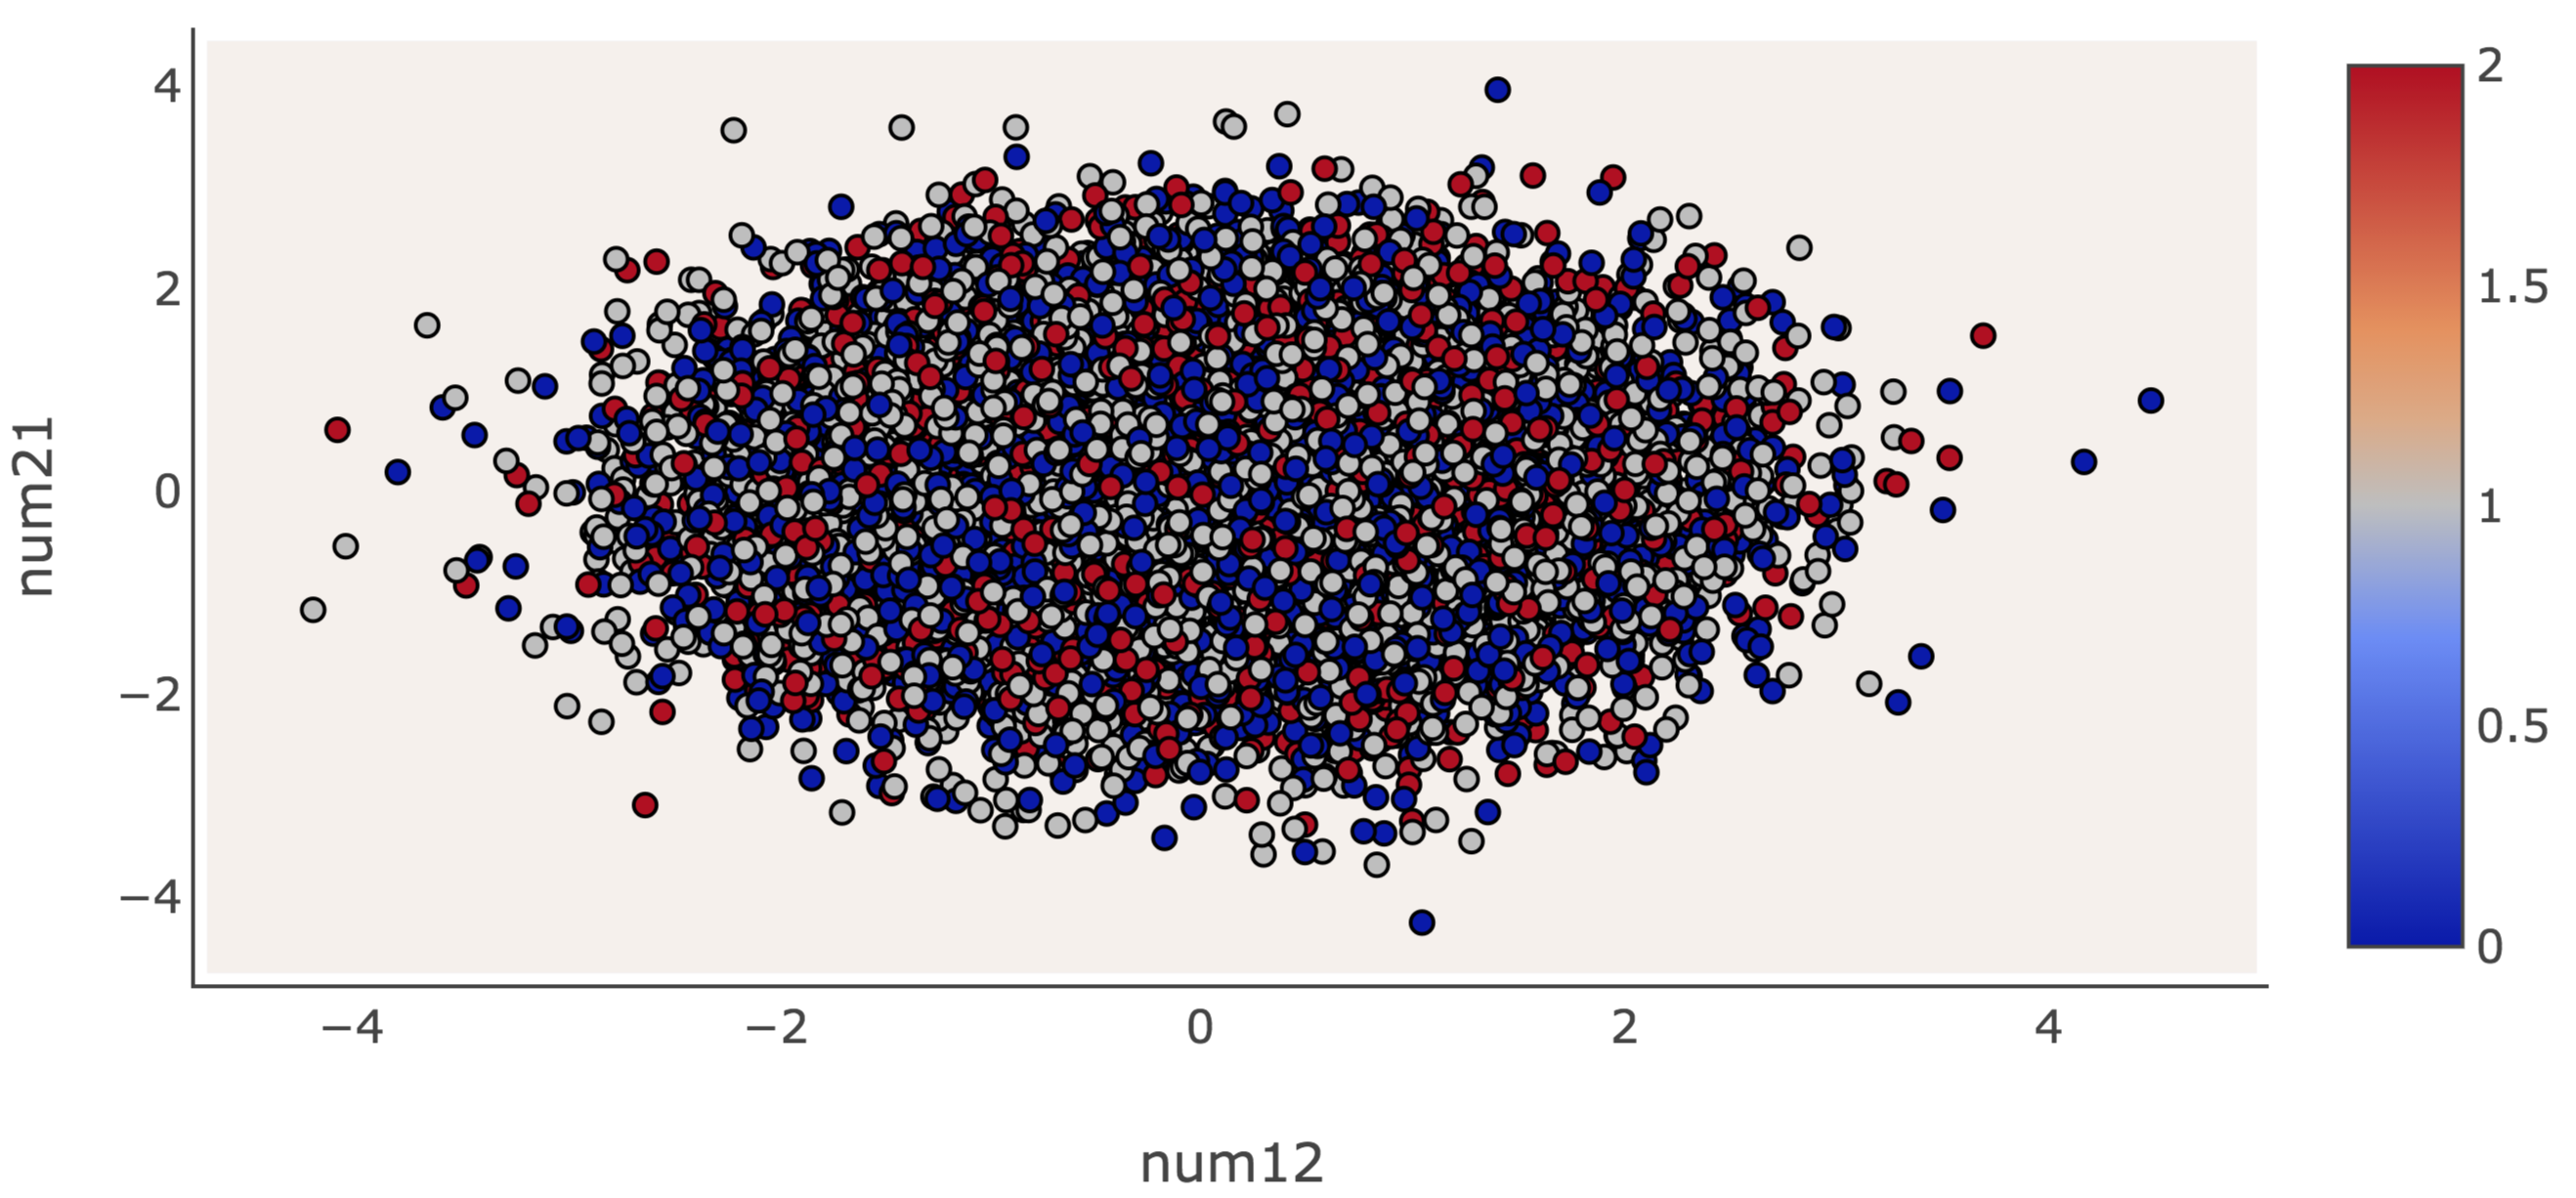
\includegraphics[width=\linewidth]{img/db_num12_num21}
			\caption{}
			\label{fig:global_db}
			\end{center}
	\end{subfigure}%
	\begin{subfigure}[tb]{.5\textwidth}
		\begin{center}
			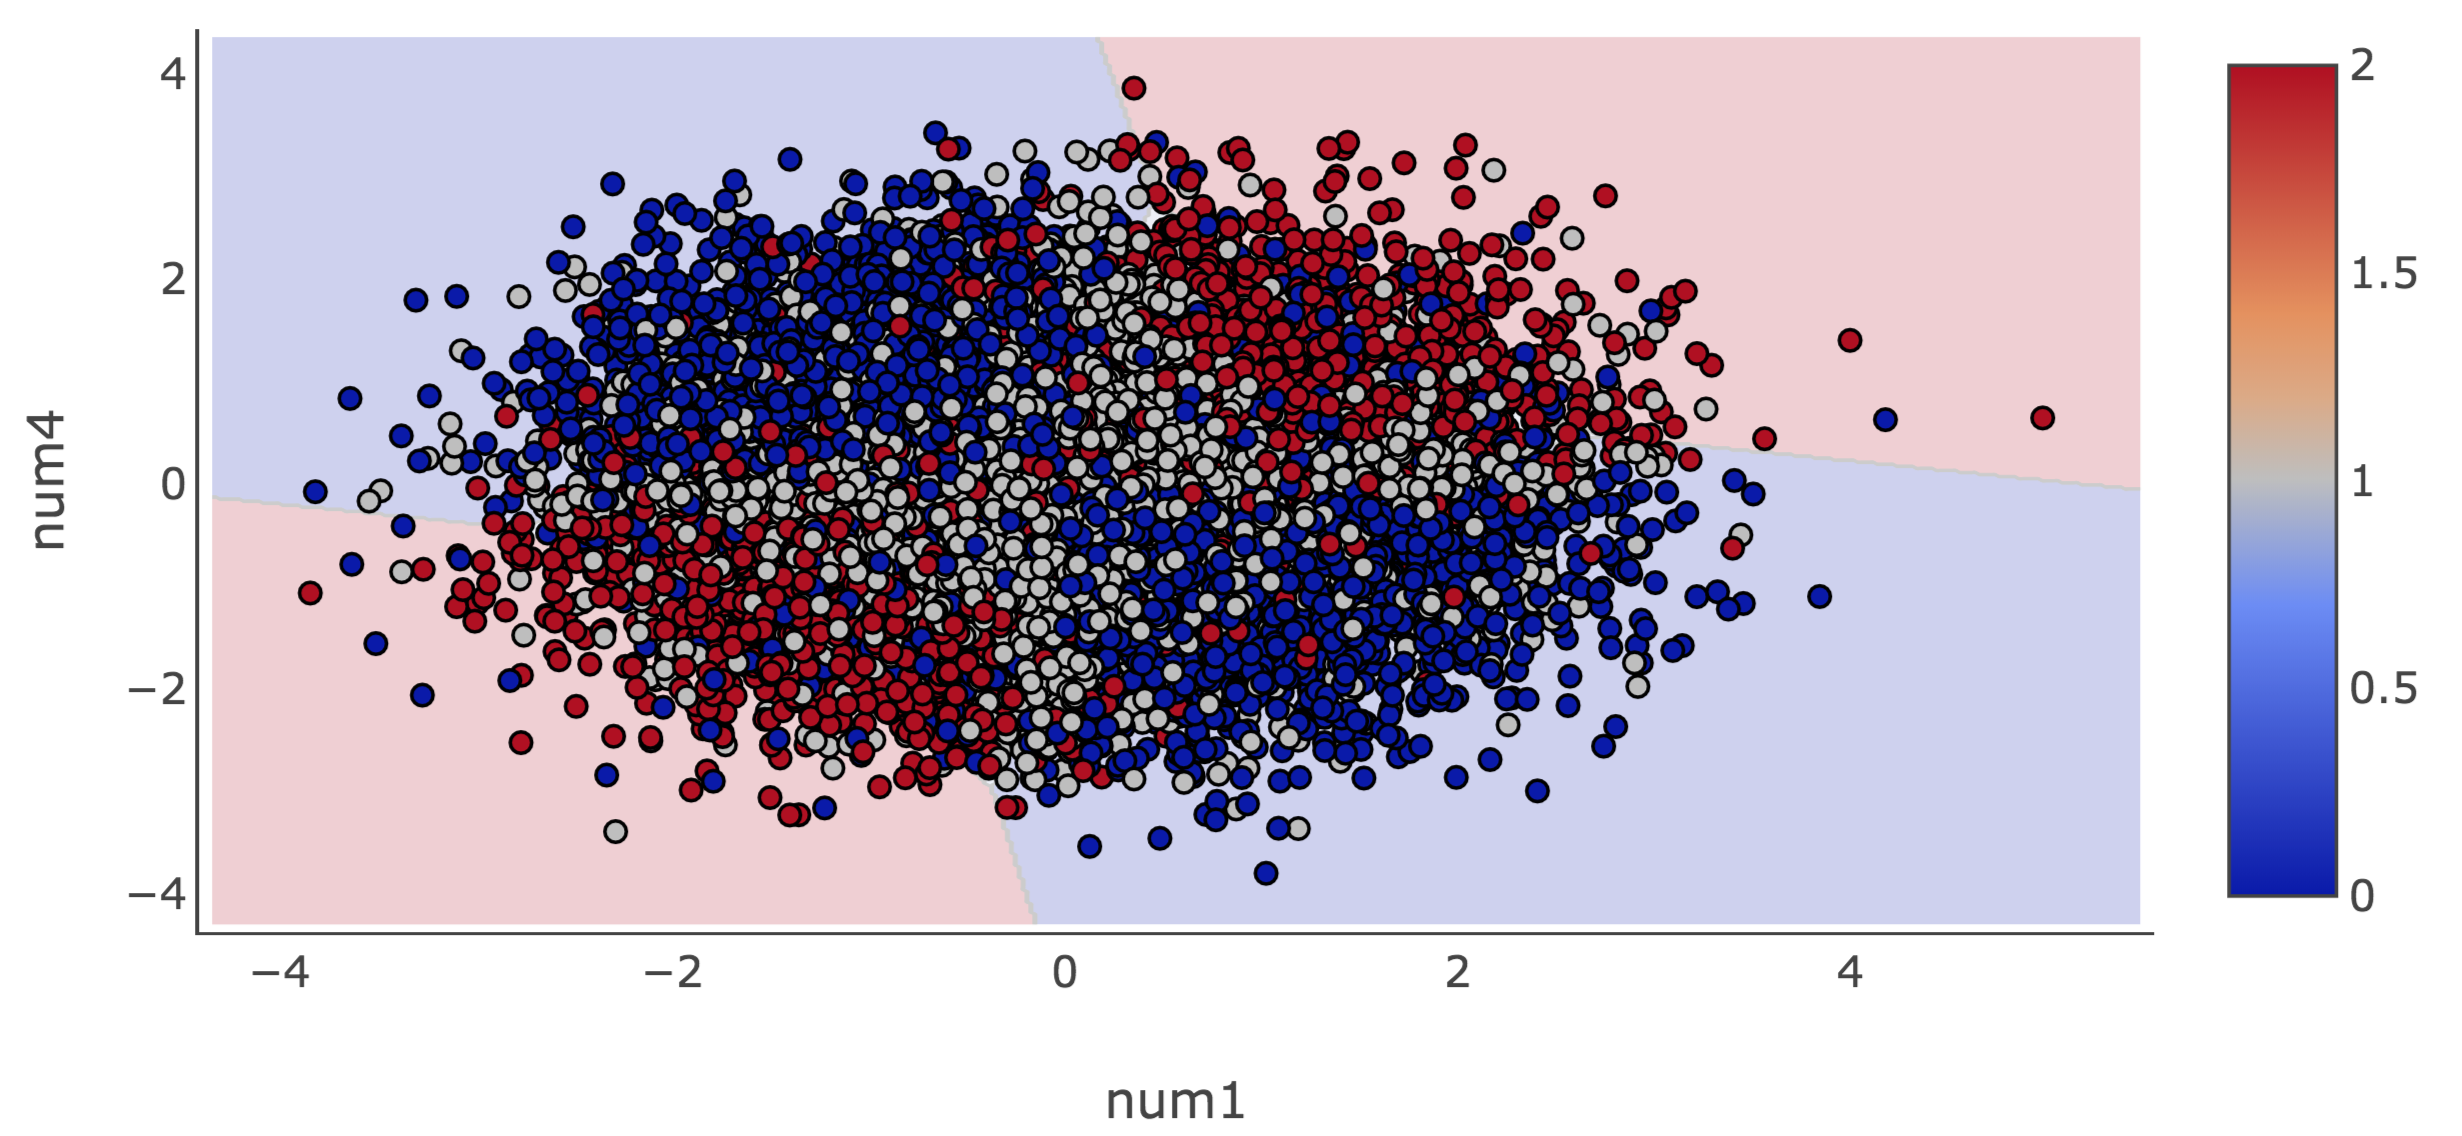
\includegraphics[width=\linewidth]{img/db_mlp_num1_num4}
			\caption{}
			\label{fig:global_db}
		\end{center}
	\end{subfigure}%
	\captionsetup{font=footnotesize}
	\caption{The color of the data points correspond to the color of the supplied ground truth labels("class1", "class 2", "class 3"). While the background color of the decision boundaries indicated class membership(i.e. separation and direction) as learned by the 
	GBM(\textbf{Figures a, b, c}). \textbf{Figure d:} Visualizes the decision boundary learned by a multi-layered MLP classifier, highlighting a different shape of the decision boundary as compared to GBM model(tree based models learn rectangular 
	boundaries.)}
\end{figure}

\subsubsection{Recommendations}
\begin{itemize}
	\item Decision Boundaries are widely used, easily understandable 2D or 3D scatter plots \cite{migut2015visualizing}
	\item Is able to show data and class membership in original feature space which is helpful in understanding feature interaction.
	\item Is model agnostic, and would work for any form of simple or complex("black box") model enabling effective model comparison.
	\item Provides the ability to instantly identify critical and cost changing data points, data elements closer to the decision boundary
	\item How do we handle high dimensional feature space \\ $\mathcal{X} \subset \mathbb{R}^P$?
	\begin{itemize}
		\item A matrix of 2D/3D decision boundary plots showing all combinations of the feature dimension. Top-K features could selected using the Shapely Feature Importance
		\item Feature Selection/Extraction techniques could be applied to reduce the high-dimensional space - e.g. RFE, NMF, PCA, CCA, LDA
	\end{itemize}
\end{itemize}


\subsection{Interpretation via Shapley Global Feature Importance}

Shapley explanations, including tree shap and even certain implementations of LIME, are a class of additive, consistent local feature contribution measures with long-standing theoretical support \cite{shapley}. Shapley explanations are the only possible locally accurate and consistent feature contribution values, meaning that Shapley explanation values for input features always sum to $g(\mathbf{x})$ and that Shapley explanation values can never decrease for some $x_j$ when $g$ is changed such that $x_j$ truly makes a stronger contribution to $g(\mathbf{x})$ \cite{shapley}. 

\begin{equation}
\label{eq:shap_additive}
\begin{aligned}
g(\mathbf{x}) = \phi_0 + \sum_{j=0}^{j=\mathcal{P} - 1} \phi_j \mathbf{z}_j
\end{aligned}
\end{equation}

\begin{equation}
\label{eq:shap_contrib}
\begin{aligned}
\phi_{j} = \sum_{S \subseteq \mathcal{P} \setminus \{j\}}\frac{|S|!(\mathcal{P} -|S| -1)!}{\mathcal{P}!}[g_x(S \cup \{j\}) - g_x(S)]
\end{aligned}
\end{equation}

Shapley values can be estimated in different ways. Tree shap is a specific implementation of Shapley explanations. It does not rely on surrogate models. Both tree shap and a related technique known as \textit{treeinterpreter} rely instead on traversing internal tree structures to estimate the impact of each $x_j$ for some $g(\mathbf{x})$ of interest \cite{tree_shap}, \cite{treeinterpreter}.

Simulated data is used to illustrate the utility of tree shap. Shapley explanations are estimated on $g_{\text{GBM}}(\mathbf{X})$ for a simulated test set $\mathbf{X}$ with known signal-generating function $f$. Results are presented in Figure \ref{fig:global_feature_imp}. Firstly, the Shapley explanations are shown globally across all class outcomes in a stacked bar chart broken down by absolute global Shapley values per class outcome. This is a good way to see a overall picture of Shapley explanations for multinomial classifiers. Secondly, the Shapley explanations are broken down per class outcome in subsequent charts. All feature contributions for $\text{num}_1, \text{num}_4, \text{num}_8$ and $\text{num}_9$ are seen as most important across all class outcomes both in the global stacked bar chart and per class outcome, which is expected based on Equation \ref{eq:f}. However, they are not seen in the same order. For example, class 0 and class 2 share the same ordering of $\text{num}_1, \text{num}_4, \text{num}_8$ and $\text{num}_9$ but class 1 does not ($\text{num}_1$ and $\text{num}_9$ are swapped). This information can be used to investigate why the Shapley explanations differ between different class outcomes at a global level.

\begin{figure}[H]
	\begin{subfigure}[tb]{.5\textwidth}
		\begin{center}
			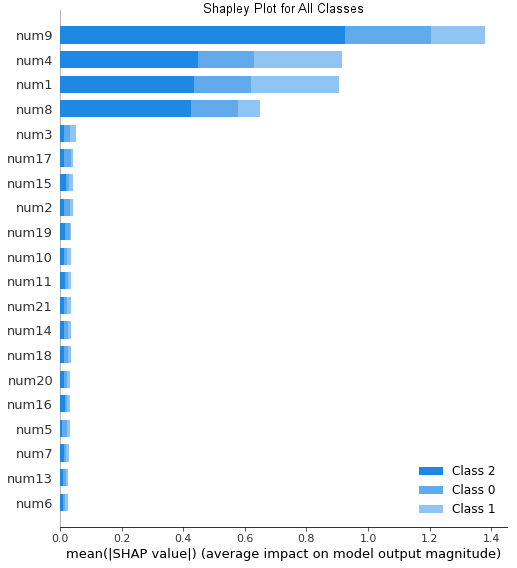
\includegraphics[width=\linewidth]{img/global_shap_sim.png}
			\caption{}
			\label{fig:global_shap}
		\end{center}
	\end{subfigure}%
	\begin{subfigure}[tb]{.5\textwidth}
		\begin{center}
			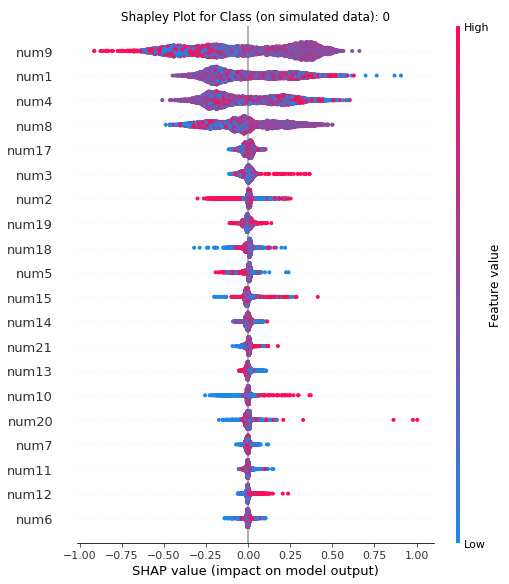
\includegraphics[width=\linewidth]{img/class_0_shap_sim.png}
			\caption{}
			\label{fig:global_shap}
		\end{center}
	\end{subfigure}%
	\vskip\baselineskip
	\begin{subfigure}[tb]{.5\textwidth}
		\begin{center}
			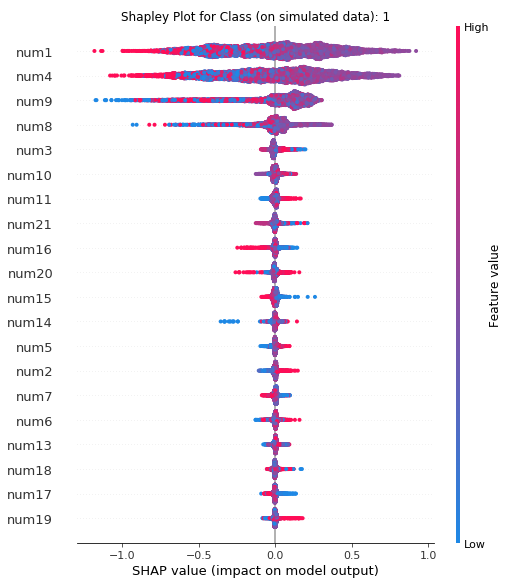
\includegraphics[width=\linewidth]{img/class_1_shap_sim.png}
			\caption{}
			\label{ffig:global_shap}
			\end{center}
	\end{subfigure}%
	\begin{subfigure}[tb]{.5\textwidth}
		\begin{center}
			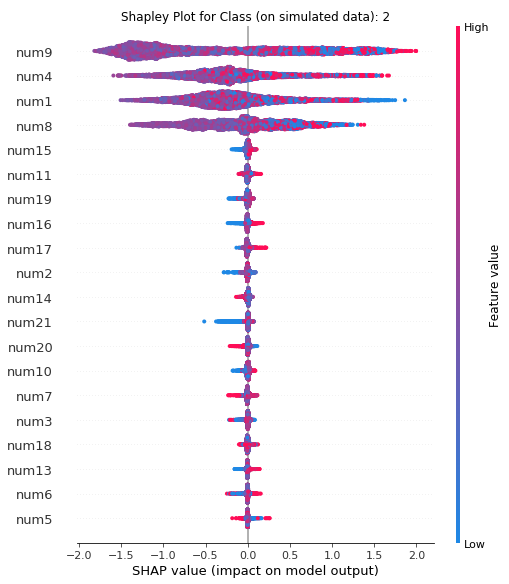
\includegraphics[width=\linewidth]{img/class_2_shap_sim.png}
			\caption{}
			\label{fig:global_shap}
		\end{center}
	\end{subfigure}%
	\captionsetup{font=footnotesize}
	\caption{}
\end{figure}

\FloatBarrier

\subsubsection{Recommendations}

\begin{itemize}
	
	\item Tree shap is ideal for estimating high-fidelity, consistent, and complete explanations of decision tree and decision tree ensemble models, perhaps even in regulated applications to generate regulator-mandated reason codes (also known as turn-down codes or adverse action codes).
	
	\item Because tree shap explanations are offsets from a global intercept, each $\phi_j$ can be interpreted as the difference in $g(\mathbf{x})$ and the average of $g(\mathbf{X})$ associated with some input feature $x_j$ \cite{molnar}. 

\item What to do if very high cardinality in response, $\mathbf{Y}$:

\begin{itemize}

  \item Examine top-K most frequent classes
  \item Examine top-K most accurate and inaccurate classes
  \item Examine classes with highest variance in sum(absolute(shap))

\end{itemize}

\end{itemize}

%\subsection{Shapley Local Feature Importance}

\subsection{Interpretation via Partial Dependence and ICE}

Partial dependence (PD) plots are a widely-used method for describing the average predictions of a complex model $g$ across some partition of data $\mathbf{X}$ for some interesting input feature $X_j$ \cite{esl}. Individual conditional expectation (ICE) plots are a newer method that describes the local behavior of $g$ for a single instance $\mathbf{x} \in \mathcal{X}$. Partial dependence and ICE can be combined in the same plot to identify interactions modeled by $g$ and to create a holistic portrait of the predictions of a complex model for some $X_j$  \cite{ice_plots}.
	
Following Friedman et al. a single feature $X_j \in \mathbf{X}$ and its complement set $\mathbf{X}_{(-j)} \in \mathbf{X}$ (where $X_j \cup \mathbf{X}_{(-j)} = \mathbf{X}$) is considered. $\text{PD}(X_j, g)$ for a given feature $X_j$ is estimated as the average output for a particular class outcome, $C'$, of the learned function $g(\mathbf{X})$ when all the components of $X_j$ are set to a constant $x \in \mathcal{X}$ and $\mathbf{X}_{(-j)}$ is left unchanged. $\text{ICE}(x_j, \mathbf{x}, g)$ for a given instance $\mathbf{x}$ and feature $x_j$ is estimated as the output for a particular class outcome, $C'$, for $g(\mathbf{x})$ when $x_j$ is set to a constant $x \in \mathcal{X}$ and all other features $\mathbf{x} \in \mathbf{X}_{(-j)}$ are left untouched. Partial dependence and ICE curves are usually plotted over some set of constants $x \in \mathcal{X}$. 

As in Section \ref{sec:surrogate_dt}, simulated data is used to highlight desirable characteristics of partial dependence and ICE plots. In Figure \ref{fig:global_pdp_ice} partial dependence and ICE at the minimum, maximum, and each decile of $g_{\text{GBM}}(\mathbf{X})$ are plotted per response outcome. The known quadratic behavior of $\text{num}_9$ is plainly visible, except for low/high value predictions across certain deciles per response outcome. When partial dependence and ICE curves diverge, this often points to an interaction that is being averaged out of the partial dependence. Given the form of Equation \ref{eq:f}, there is a known interaction between $\text{num}_9$ and $\text{num}_8$. Combining the information from partial dependence and ICE plots with $h_{tree}$ can help elucidate more detailed information about modeled interactions in $g$.

\begin{figure}[H]
	\begin{subfigure}[tb]{.5\textwidth}
		\begin{center}
			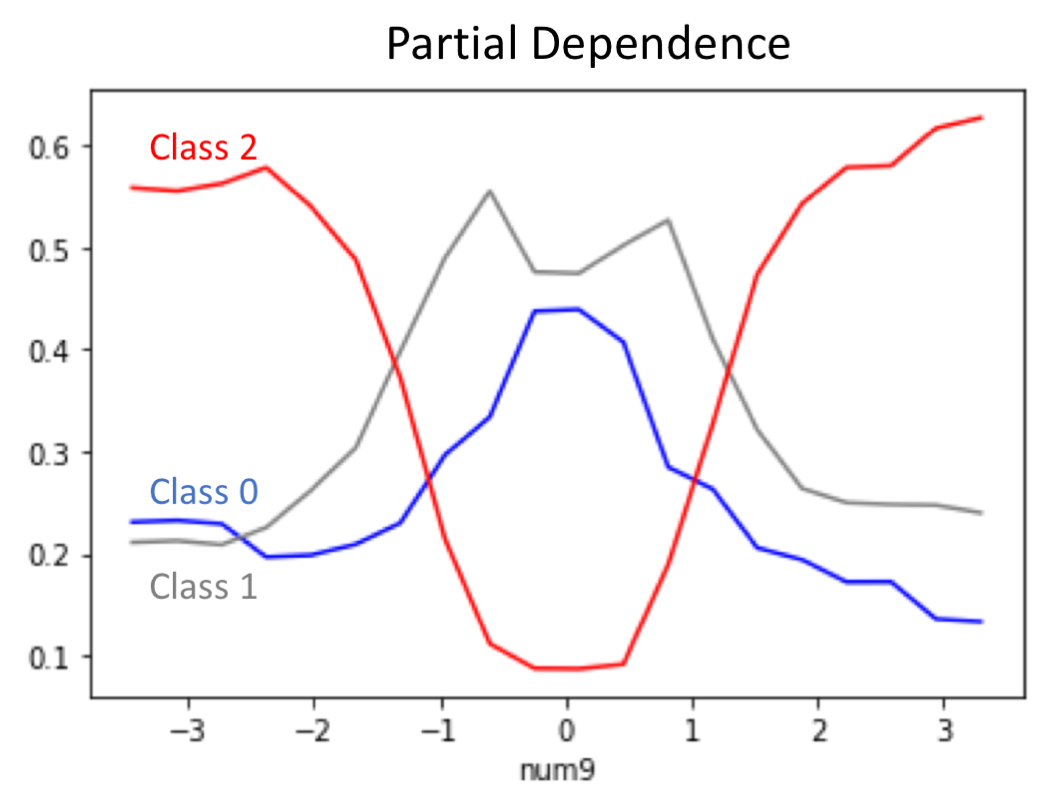
\includegraphics[width=\linewidth]{img/pdp_ice_sim_annotated_a.png}
			\caption{}
			\label{fig:global_shap}
		\end{center}
	\end{subfigure}%
	\begin{subfigure}[tb]{.5\textwidth}
		\begin{center}
			\includegraphics[width=\linewidth]{img/pdp_ice_sim_annotated_b.png}
			\caption{}
			\label{fig:global_shap}
		\end{center}
	\end{subfigure}%
\end{figure}

\FloatBarrier

\subsubsection{Recommendations}

\begin{itemize}

\item Combining $h_{\text{tree}}$ with partial dependence and ICE curves per class outcome is a convenient method for detecting, confirming, and understanding important interactions in $g$.

\item What to do if very high cardinality in response, $\mathbf{Y}$:

\begin{itemize}

  \item Examine top-K most frequent classes
  \item Examine top-K most accurate and inaccurate classes
  \item Examine classes with highest variance in partial dependence
  \item Examine classes with largest differences between partial dependence and ICE
  
\end{itemize}

\end{itemize}

\section{Supplementary Materials}

% Credit card use case, alternate figure

UCI credit card dataset \cite{uci}.

\begin{center}
  \url{https://github.com/navdeep-G/interpretable-ml/tree/master/notebooks/credit/multinomial}
\end{center}

%\section{Credit Card Data Use Case}
%\subsection{Global Analysis}
%\subsubsection{Decision Tree Surrogate}
%\subsubsection{Decision Boundary Plots}
%\subsubsection{Shapley Global Feature Importance}
%\subsubsection{Partial Dependence and ICE}
%\subsection{Local Analysis: Local Shapley Feature Importance}

\section{Conclusion}

\subsubsection*{Acknowledgments}
Use unnumbered third level headings for the acknowledgments. All
acknowledgments go at the end of the paper. Do not include
acknowledgments in the anonymized submission, only in the final paper.

%-------------------------------------------------------------------------------
%\section{References}
%-------------------------------------------------------------------------------

\bibliographystyle{plain}
\bibliography{nips_multinomial_2018}
\end{document}